\chapter{Overture}\label{chap:intro}
\openepigraph{Écho. Citer ceux du Panthéon et du pont de Neuilly. }{Gustave Flaubert, Dictionnaire des idées reçues}
\openepigraph{Echoes shows the direction that we’re moving in. }{David Gilmour, about the making of ``The Dark Side Of The Moon''}

\vspace{-2.5em}
\marginpar{%
    \footnotesize
    \textbf{Resources:}
    \begin{itemize}
        \item[\faYoutube] \href{https://www.youtube.com/watch?v=lLUcOFwZvyY&t=22s}{Testing The World's Longest Echo}
        \item[\faYoutube] \href{https://www.youtube.com/watch?v=px3oVGXr4mo}{SKUNK BEAR : What Does Sound Look Like?}
        \item[\faYoutube] \href{https://www.youtube.com/watch?v=ZwgovJSQ5UM}{ARTE : La Magie Du Son}
        \item[\faYoutube] \href{https://www.youtube.com/watch?v=uH0aihGWB8U&t=631s}{Daniel Kish: How I use sonar to navigate the world}
    \end{itemize}

}


\def\MyText{\textsc{Echoooes}}
\newcommand\mytext[2][black]{\scalebox{#2}{\textcolor{#1}{\MyText}}}

% This thesis is about taking inspiration from people, bats, Daredevil and Pink Floyd.
\newthought{In a nutshell,} this \PhD/ thesis is about acoustic
\stackinset{c}{4ex}{c}{ 1.4ex}{\mytext[black!70]{.8}}{%
\stackinset{c}{2ex}{c}{ 3.2ex}{\mytext[black!25]{.7}}{%
\stackinset{c}{3ex}{c}{-1.3ex}{\mytext[black!35]{.9}}{%
\mytext{1}%
}}}.
\\We live immersed in a complex acoustical world, where every concrete thing can sound, resound and echo.
For humans it is difficult to imaging sound, its constituents and its generation.
In fact, it is processed by our auditory systems and brain so efficiently that our attention is detached from the physical laws governing it.
Therefore, when listening to something, we unconsciously focus on its \textit{content}.
% When we listen to music, we focus on the melody in the music; when listen to speech, we focus on the words;
% when something is smashed to the ground, we may be able to guess what ``was'' it.
% \\However not only \textit{semantic information} about the source is carried by the sound.
% There are many other types of information that we retrieve and infer from it, such as \textit{temporal} and \textit{spatial} information.
% For instance, we are able to localize its source:
% if someone is calling us, we unconsciously know towards where to turn.
% We can guess if an noisy motorbike is approaching or moving away.
% Another striking example, which involves simple math, is estimating of how far the storm is, simply counting the time between a view a lightning a listening to thunder.
% We can even guess the size and the type of the room we are currently sitting in.
\\Evolution lead us to conduct this process without any efforts, despite the presence of huge level of background noise, for instance in a during a concert.
This outstanding capability is not limited to humans and is common to all the creatures we are sharing the physical world with.

\mynewline
We process all the information of the complex \textit{acoustic scene} surrounding us.
While reaching the ears, sound propagates in all direction and portion of its energy arrives to us directly, other indirectly after being reflected around.
This process leads to the creation of \textit{echoes} and \textit{reverberation}.
Typical examples are the echoes produced by huge rocky mountains or by huge walls in monumental buildings, such as the Panthéon in Rome or the pont de Neuilly in Paris.
Echoes refers to that particular reflected sound which can be hear distinctly, thus, characterized by specific time of arrival and attenuation.
In smaller environments, echoes are still present but are typically less perceived as they arrive more quickly and densely.
What is then perceived here is the so called reverberation, which happen in empty rooms or churches.

\mynewline
Some animals are evolved to ``see'' through echoes.
For instance, the two (of the most) striking examples are bats and whales which use them as navigation and foraging mechanism.
By emitting sound patterns and listening the echoes that return form the environmental, these animals scan the surrounding space, identify and locate objects.
Just like an active sonar, here the echoes are voluntarily produced and this is referred to as \textit{active echo-location}.
As opposed to, in \textit{passive echo-location} the source sound is not emitted, but rather only received.
\marginpar{
    \footnotesize
    This technique is developed instinctively by some blind people as well.
    By tapping their canes or clicking their tongues, they are able to avoid obstacles when walking.
    French philosopher Denis Diderot in 18th century recorded the this incredible ability, which was labeled as ``echo-location'' only 300 years later by Donald Griffin.
}.
``Locating it'' means estimating its delay with respect to the direct sound.
These delay can be converted into distances, in the same as our grandparent taught us to localize storm by counting the time between a lightning and its thunder.
That is how bats and whales find preys, see obstacles and orientated in dark caves.
However, the term ``echo-location'' here could be misleading as it may refer to the only problem of locating objects.
As we will discuss later, the application goes beyond to simply localization.
Therefore, in this thesis it will change it in favor of \textit{echo estimation}.

\mynewline
Remarkable examples of passive echo estimation in nature are not very known.
Sand scorpions uses the propagation of vibration in sand to localize their prays at night.
By deploying their 8 legs in particular configurations, they perform passive (seismic) echo-location.
This technique is common to spiders who sense to the reverberation in their complex web\sidenote{
    According to some recent reseach studies, spiders appear to offload cognitive tasks to their webs.
    The web may acts then as a complex system processing and filtering the information, which are then returned to their owner.
    \citeonly{sokol2017thoughts}
}.
They are not only able to localize the preys fast, but also identify them, and disambiguate from simple objects move by the wind.
For some species, this task is performed by sensing the web with only one leg.
In this case, instead of emitting sound, evolution taught them to uses complex structures (for scorpions legs configuration, for spiders webs shapes)
in order to procure food.

\mynewline
Echoes do not only serve for computing distances or localizing preys.
For instance, they make speech more intelligible and provide music with ``dimensionality''\citeonly{sacks2014musicofilia}.
This phenomenon is material of studied in \textit{room acoustics} and it is applied for designing theatres, auditoriums and meeting rooms, whose actual propose is listen well.
In the same context, echoes may be used as tool for acoustic measurement, to study the acoustic quality of an environment, sometimes referred to as its \textit{coloration}.

\mynewline
To conclude with, this thesis is focused on both how to estimate passively acoustic echoes and why they helps audio analysis.
It does not cover echo-aware audio synthesis, that is or provide dimensionality to produced music

\mynewline
One may ask, what does it mean, to estimate echoes and use them?
Therefore with echo estimation we will refer to the estimation of them both.
Even there are less clear example in nature to explain it, passive echo location is used by our mind instinctively in order to process the acoustic scene.

\mynewline
Therefore, in the context of computer science, it is natural to ask ourself how we can build machine that can listen as we do?
In order to process sounds, machines and computer use algorithmic tools which fall in the research field of \textit{audio signal processing}.
How is it implemented? it will be outlined in the next section.
How echoes can help such processing? it will be explained immediately after.

\section{Echo-aware Signal Processing for Audio Scene Analysis}\label{sec:intro:problem}
The problems addressed in this thesis are indicated in the thesis title: \textit{Echo-aware signal processing for audio scene analysis}.
There are two parts in the sentence that deserve an explanation: \textit{echo-aware signal processing} and \textit{audio scene analysis}.
Let us start from the second one which provide the general context.

\subsection{Audio scene analysis}
Sounds carry information about sound sources.

Information about the \textit{content} and the \textit{nature} of the sound.
But other information as well.

\newthought{Audio Scene Analysis}
\newthought{Audio Scene Synthesis}


\subsection{Echo-aware signal processing}
\textit{Signal processing} is the process of analyzing and modifying a \textit{signals}, which are mathematical representation of quantities carrying information about a phenomenon.
When this signals represents sound, such as music or speech, then we speak about \textit{sound} or \textit{audio signal processing}.
\marginpar{
    \footnotesize
    \textit{Audio is a more technical term, referring to sound coming from a recording, transmission or electronic device.
    Sound is a more generic word and can be caused by any source.}
}
\textit{Audio signal processing} involves applying various mathematical and computational techniques to analog and digital signals.
There are multiple reasons to do this, such as produce new signals with higher quality than the original signal and extract high-level information the signal carries.
In order to achieve this, complex system are built which can be represented as collection of simpler subsystems, with well-defined tasks, interacting with each other.
In (audio) signal processing, these subsystems roughly fall into four categories: \textit{representation}, \textit{enhancement}, \textit{estimation}, and \textit{adaptive processing}.
Many related problems can be then decomposed into blocks that belong to one of more of these categories.

\begin{description}
    \item[Representation] Signal can be represented and described in many different way.
    Through different representations, the \textit{information} contained in the signals becomes more relevant and suitable for certain tasks than other.
    \\Representation can be lossy or lossless, and are generally implemented through change of \textit{domain} or \textit{feature}.
    The most famous representation in case of audio is the Fourier basis which change the signal domain from from time to frequencies.
    The process of changing representation is often called: \textit{analysis} and \textit{synthesis}.

    \item[Enhancement] Measurement are affected by noise and interferences which corrupt and hide relevant information, making its retrieval harder and sometimes impossible.
    Therefore, signal enhancement, that is removing noise, is typically a necessary step.
    \\Enhancement constitute a huge dome of methods:
    form simple denoising by averaging of repeated measurement to huge system based on neural network.

    \item[Estimation] Often we wish to estimate some key properties of the target signal which may be used as inputs to a different algorithm.

    \item[Adaptive processing] deals with adaptive algorithms and filters controlled by variable parameters.
    A common means to adjust those parameters according to an optimization algorithm which rely on statistical properties of the signal of interest.
    They often implement a kind of online optimization where an objective function is being minimized.
    When new data is observed, its discrepancy with the current estimate is used to produce a new estimate in a way that reduces the objective.
\end{description}


That is being said, the goal of this thesis is to improve the above state of in indoor audio signal processing along two axes:
First, by deepening our understanding of acoustic echoes, provide new methodologies to estimate them surpassing the limits of current approaches.
Second, by extending previous echo-aware methods, show how typical audio application can benefits of prior knowledge of these elements of acoustic propagation.
\mynewline
To that end, the dissertation demonstrates two claims:
\begin{enumerate}
    \item Acoustic echoes can be estimated blindly from microphone recordings;
    \item Typical audio scene analysis and audio processing methods can take advantage of acoustic echoes, by easily integrating their knowledge in standard algorithms.
\end{enumerate}


Based on this idea, so-called \textit{echo-aware} methods have been introduced few decades ago, where matched filters (or rake receivers) are used to constructively sum the sound reflections \citeonly{Jan1995matched, Affes1997signal} and build beamformers achieving much better sound qualities \citeonly{gannot2001signal}. This methods have recently regained interested as manifested by the European project SCENIC~\citeonly{Annibale2011scenic} and the UK research \href{http://www.s3a-spatialaudio.org/}{S$^3$A project}. They show that knowing the properties of a few early echoes can boosts performances of typical indoor audio inverse problems such as speech enhancement (SE) \citeonly{Dockmanic2015raking, Kowalczyk2019raking}, sound source localization \citeonly{ribeiro2010turning, DiCarlo2019mirage}, and separation \citeonly{scheibler2017separake, leglaive2016multichannel}.
Another fervent area of research spanning transversely the audio and acoustic signal processing fields is estimating the room geometry blindly from acoustic signals. As presented by Crocco \textit{et al.} in \citeonly{crocco2017uncalibrated}, the end-to-end room geometry estimation (RooGE) involves many subsequent subtasks: RIR estimation, peak picking, microphones calibration, echo labeling, reflectors estimation. Acoustic echo retrieval (AER) is common to many of these topics. It consists in estimating the properties of echoes such as their TOAs and energies. The former problem is referred to as TOA estimation, or time-delay estimation when the direct-path is taken as reference. Furthermore, as interesting applications, these methods have been recently used in active scenarios, namely knowing the transmitted signals, using unmanned aerial vehicle (UAV, a.k.a. drones) \citeonly{jensen2019method, Boutin2020drone} and mobile-phones \citeonly{Shih2019phone}.



% \newthought{Audio Signal Processing}
% \begin{itemize}
%     \item Motivation
%     \item Definitions, Function, Characteristics
%     \item Current challenges
% \end{itemize}

% \newthought{Inverse Problem}
% Starting with the effects to discover the causes has concerned physicists for centuries.

% While in many ways, mixtures are not different to any other audio signal, two research questions stand out prominently: • Can we obtain the sources sj from the mixture x? • Can we find the number of sources J from x? These two questions are addressed in the scientific fields of sound
% source separation and source count estimation


% Inverse problems appear when we want to see or examine something that we cannot access directly. What we have is an indirect measurement that contains hidden information.

% An inverse problem is always a counterpart of a direct problem, as shown in the schematic diagram below. The direct problem is going from object to data, and the inverse problem is about finding the object back from the data.

% The assumed few thousand taps. This model was very popular in the early stages of research [48]–[55]. Recently, interest has revived with sparse penalties which account for prior knowledge about the physical properties of AIRs, namely the facts that power concentrates in the direct path and the first early echoes [56]– [60] and that the time envelope decays exponentially [61], but these penalties have not yet been used in a BSS context.


\section{Audio Inverse Problems}\label{sec:processing:inverse}
\cite{kitic2015cosparse}
\openepigraph{Their generality is of such a wide scope that onemayeven argue that solving inverse problems is what signal processing is all about}{Srdan Kiti\'c, \textit{Cosparse regularization of physics-driven inverse problems}}
\openepigraph{everything is an optimization problem}{\citeonly{watson2001nonlinear}}
\marginpar{
    \footnotesize
    One can see the paralelism with the engineering concepts: analysis and sythesis.
}
In~\cref{sec:intro:problem} we have informally defined \textit{inverse problems}, with an emphasis on inverse problems in signal processing.
An inverse problem is a type of a mathematical problem where we start with the observations and we want to estimate model parameters that produced them.
\\Inverse problems pervades all the field of science and engineering:
source localization~\cite{},
image processing~\cite{},
acoustic imaging and tomography~\cite{},
\marginpar{
    \footnotesize
    A historical example are the calculation of the Earth circunference by Eratosthenes in III century b.c.\\
    and the calculations of Adams and Le Verrier which led to the discovery of Neptune from the perturbed trajectory of Uranus.
}

A inverse problems is defined as the counterpart of a \textit{forward}\sidenote{often referred to as \textit{direct}} problem.
Without falling in and deep mathematical formalism and taxonomies which can be found in \citeonly{bal2012introduction},
we will simply consider the following informal definition:
\begin{center}
    \textit{\emph{Forward problem} starts from known input, while \emph{inverse problem} starts from known output~\cite{santamarina2005discrete}.}
\end{center}
Both these problems focus on an operation relating maps objects of interest, called \textit{parameters} or \textit{variables},
to information collected about these objects, called \textit{measurements}, \textit{data} or \textit{observation}.

For instance, in our context, the direct problem may be the estimation of the \RIR/(s) starting from the known room parameters,
and, the related inverse problem would be the estimation of such room properties from the observation of the \RIR/(s).

Formally, a forward problem is defined through a mathematical model, described by a \textit{operation} $\scrM(\cdot)$
mapping \textit{parameters} $x \in \scrX$ to the \textit{observation} (or measurement) $y \in \scrY$:
\begin{equation}\label{eq:processing:model}
    y = \scrM(x)
    .
\end{equation}
Then, the inverse problem defines a method $\kinv{\scrM}$ that ``reverts'' $\scrM$ in order to recover (estimate) $x$ form the observation of $y$.
% The operator $\scrM$ describes our best effort to construct a \textit{model} for the available data $y$.
% The choice of $\scrX$ describes our best effort to characterize the space where we believe the parameters belong.

As discussed in~\cite{bal2012introduction}, \textit{solving} the inverse problem consists in finding point(s) $x \in \scrX$ from (knowledge of) data $y \in \scrY$
such that~\cref{eq:processing:model} or an approximation of~\cref{eq:processing:model} holds.
Under this light, the operator $\scrM$ ant the choice of $\scrX$ describes our best effort to construct a \textit{model} for the data $y$ and
the space where the parameters $x$ belong, respectively.
\marginpar{
    \footnotesize
    one can already see the paralelism the the definition of the mixing process defined in~\cref{sec:intro:problem}
}

\textsc{For instance, in Case of} \textit{linear} inverse problem, and for $\scrY$ and $\scrX$ being vector spaces of dimensions $M$ and $N$ respectively,
then the forward map can be written as a linear system:
\begin{equation}\label{eq:processing:linear_forward}
    \bfy = \bfM \bfx
\end{equation}
where $\bfM$ being a matrix, namely the operator $\scrM$ becomes a matrix multiplication by $M$.
It follows that the inverse map associated to~\cref{eq:processing:linear_forward} is the application of the inverse matrix $\kinv{M}$.
% While solving a direct problem the an operator needs to be found, in solving the inverse one either the operator is known and needs
% to be $reverts$t

Typically, forward problems are considered somehow the ``easier''.
In fact, even in the observation model $\scrM$ is known perfectly, it is not always possible to find its counterpart.
This because of
\begin{itemize}
    \item presence of \textit{noise} in the measurement which are not always additive and statistically independent \wrt/ $x$.
    \item the problem is \textit{well-posed} and \textit{well-conditioned}, namely $\scrM$ needs be injective and stable.
    In other words, some information is recoverable, other is completely lost, other highly sensible to noise
    \sidenote{
        \textbf{injective} ensure the uniqueness of the solution, while \textbf{stability}
        ensure a continuity on the data.
        These are known as the Hadamard's \textit{solvability conditions}.
    }.
\end{itemize}

As we could images, many interesting and fundamental inverse problem are
\textit{ill-posed} or \textit{ill-conditioned} in general, even in the following ``simple'' ones~\cite{kitic2015cosparse}:
The solution to the deconvolution problem, where the direct inversion of the transfer function results in instabilities
at high frequency; and the solution a linear system $\bfy = \bfM \bfx$ where $\bfM$ is invertible
may lead to erroneous results and numerical instabilities.

Therefore, sometimes ones have to settle for restring the set of solution $\scrC \subset \scrX$,
where $\scrM$ is stable and injective\sidenote{This framework was originally proposed by Tikhonov.}.
Promoting solution $x \in \scrC$ is can be achieved through \textit{model priors}, namely prior knowledge about solution, which can
be classified in the following methodologies:
the usage of \textit{geometric constraints} that deterministically define the solutions; the imposition of \textit{penalization}
which ``promotes'' solution of a certain shape (\eg/ \textit{sparse}
\sidenote{\textbf{sparsity} is a fundamental concept of this thesis, better discussed in~\cref{pt:estimation}
} or \textit{smoothness});
and casting the problem in a \textit{bayesian framework} which versatilely incorporate prior and posterior density function describing the data.

Let us give two example of practical systems that will be recurrent thought out the entire thesis.

\subsection{Selected Audio Inverse Problems}
Here follow some famous problems in the field of audio signal processing with application to speech, music and environmental audio.
Given the mixing process defined in~\cref{sec:processing:model},

% \begin{description}
%     \item[sound source separation and enhancements] as the problem of retrieving a (set of) source signal from a mixture.
%     \item[sound source localization] estimation of source location from the observation of the sound production.
%     This has sense as long as the impulse response convey space properties.
%     \item[microphones calibration] estimation of the microphone placement.
%     \item[\RIR/ estimation] estimation of the filters.
%     Blind Channel Estimation or System Identification.
%     \item[Acoustic Echoes Estimation] estimation of the filters
%     \item[dereverberation] estimation of the filters
%     \item[room geometry estimation] estimation of the room
%     \item[automatich speech recognition]
% \end{description}

\begin{table}[!h]

    \begin{fullwidth}
    \centering
    \small

    \begin{tabular}{p{0.33\linewidth}|p{0.66\linewidth}}
    \toprule
    Inverse Problem & \textit{Can we estimate the...} \\
    \hline
    Audio Source Separation  & the signal of the sources $s_{j}$ from the mixture $\boldsymbol{x}$? \\

    Sound Source Localization & the position $\mathbf{s}_{j} \ =\ [ x_{s_{j}} ,\ y_{s_{j}} ,\ z_{s_{j}}]$  of the source $s_{j}$ from the mixture $\boldsymbol{x}$$ $? \\

    Microphone (Array) Calibration & the position of the microphone (array) position $\mathbf{x}$ from the mixture $\boldsymbol{x}$? \\

    \RIR/ Estimation & the filter between the sources $\boldsymbol{s}_{j}$ and the mixture $\boldsymbol{x}$ from $\boldsymbol{x}$? \\

    Room Geometry Estimation & the shape of the room in which the mixture $\boldsymbol{x}$ recoding source $s_{j}$? \\
    \bottomrule
\end{tabular}
    \caption{Selected audio inverse problems}
    \label{tab:processing:problems}

    \end{fullwidth}


\end{table}

\openepigraph{Everything is connected}{Douglas Adams, \textit{Dirk Gently's Holistic Detective Agency}}
\newthought{Depending on the scenario}, all these problems exhibits strong inter-connections,
namely the solution of one may be (dependent on) the solution of another.
Therefore, exploiting expertise and knowledge,
interconnect and hierarchical approaches may be built\sidenote{Machine Learing allows now for end2end approaches}:
for instance, many spatial filtering techniques used for \SE/ rely on \SSL/ blocks;
and in order to achieves \RooGE/, \AER/ must be done.



\section{Thesis Outline and Main Contributions}

The dissertation is broken into three largely parts which are largely interconnect, as show in the~\cref{fig:intro:thesis_mindmap}:

\begin{figure}[t]
    \begin{sidecaption}[Thesis Organization]{%
        Schematic rganization of the thesis, dependecies between chapters linked to author contributions.
    }[fig:intro:thesis_mindmap]
    \centering
    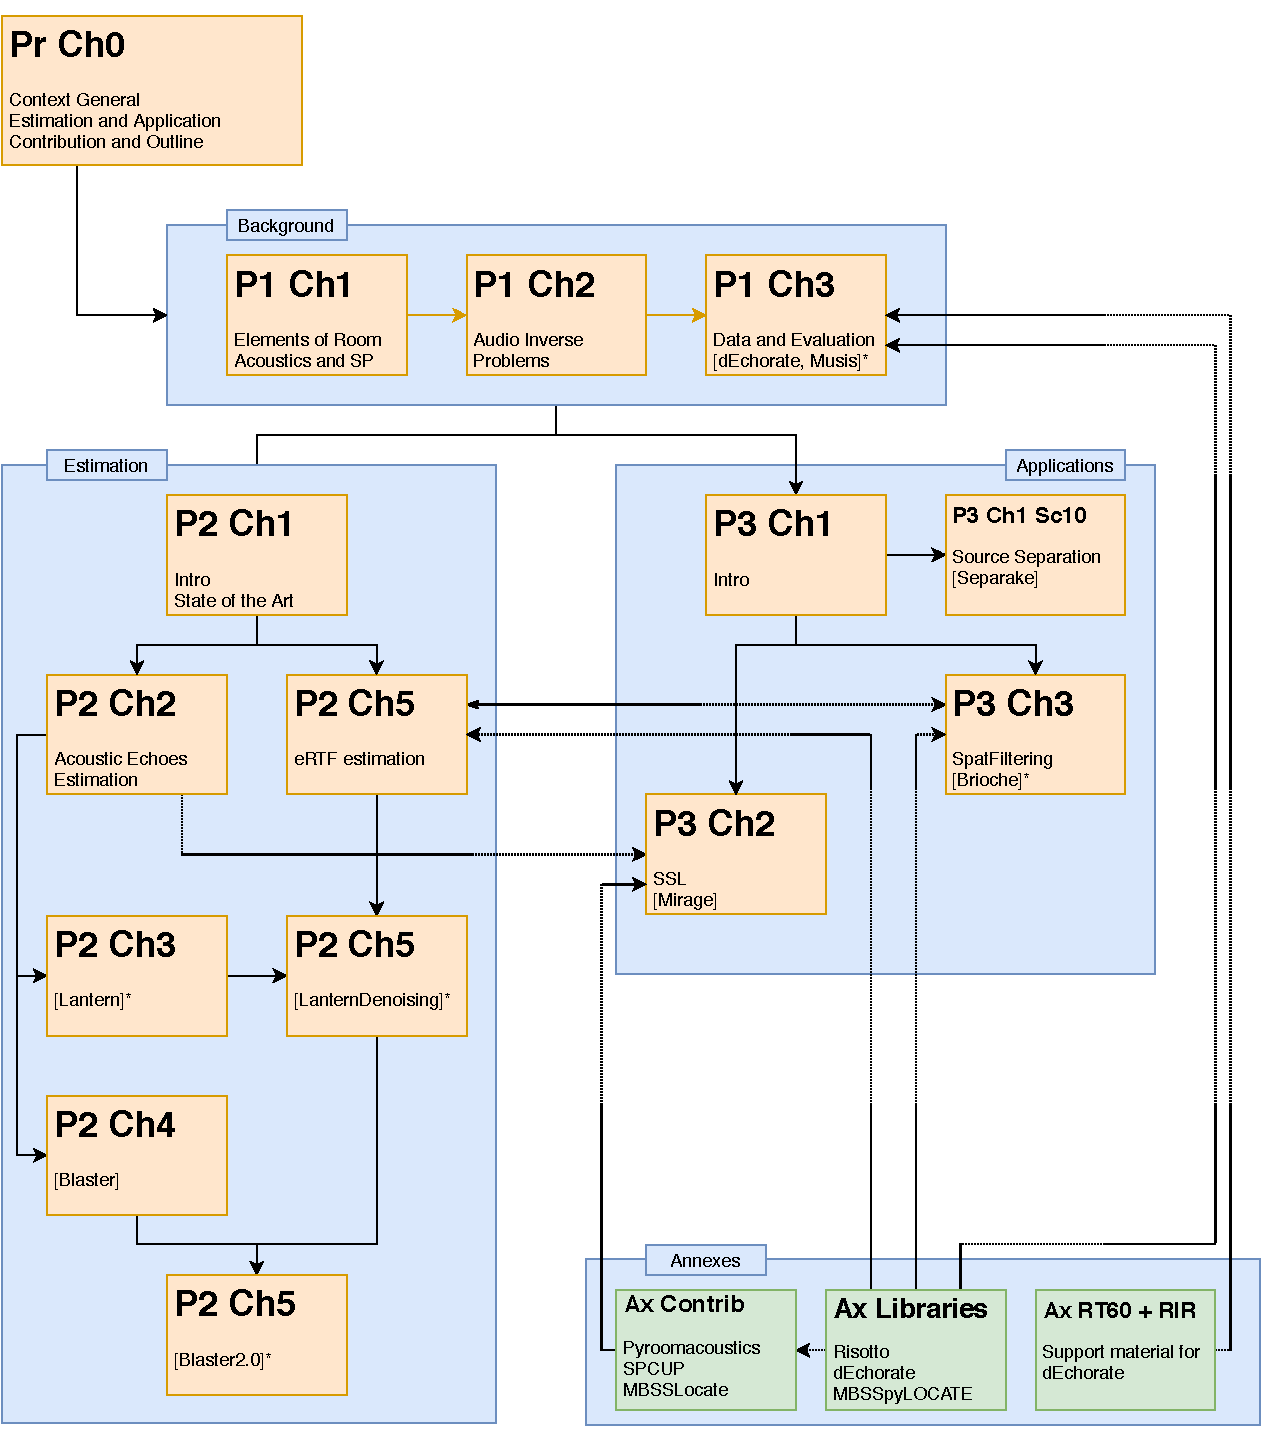
\includegraphics[width=\linewidth]{intro/thesis_mindmap.pdf}
    \end{sidecaption}
\end{figure}


\newthoughtpar{Room Acoustic meets Signal Processing}
\begin{description}
    \item[\cref{ch:acoustics}]\synopsisChAcoustics
    \item[\cref{ch:processing}]\synopsisChProcessing
\end{description}

\newthoughtpar{Acoustic Echoes Estimation}
\begin{description}
    \item[\cref{ch:estimation}]\synopsisChEstimation
    \item[\cref{ch:lantern}]\blindtext[1]
    \item[\cref{ch:blaster}]\blindtext[1]
    \item[\cref{ch:blasterr}]\blindtext[1]
\end{description}


\newthoughtpar{Echo-aware Audio Scene Analysis}
\begin{description}
\item[\cref{ch:application}]\blindtext[1]
\item[\cref{ch:separake}]\blindtext[1]
\item[\cref{ch:mirage}]\blindtext[1]
\item[\cref{ch:brioche}]\blindtext[1]
\end{description}

\section{List of Contribution}
This dissertation draws heavily on the earlier work and writing in the following papers, written jointly with several collaborators:

\begin{itemize}
    \item \fullcite{di2021dechorate}
    \item \fullcite{di2020blaster}
    \item \fullcite{di2019mirage}
    \item \fullcite{deleforge2019audio}
    \item \fullcite{lebarbenchon2018evaluation}
    \item \fullcite{scheibler2018separake}
\end{itemize}


\section{Don't Panic!}
The reader will have already noticed that a large margin is left free on the right side of each page of the manuscript.
We will use it to insert comments, historical notes as well as figures and tables to complete the subject.
This graphic charter is inspired by the work of Tufte (2001) and produced using the latex tufte-latex class.
We emphasize that the presence of the clickable GitHub logo in the margin indicates the online availability of the codes.

\subsection{Quick vademecum} for the readers:
\begin{itemize}
    \item Bibliographic references are denoted as \cite{kuttruff2016room}.
    \item Figures, Tables and other floating objects as well as equations are numbered within the chapter number.
    \item Equations are referred as~\cref{eq:acoustics:green_definition}
    \item The main matter of the Thesis’s manuscript starts at page 1, until page 103.
    \item The back matter covers the list of the candidate’s publications and the bibiographic references cited along the text.
    \item Small notes on the margin might be used to easily navigate through the Example of margin note manuscript. They are meant to summarize paragraphs/blocks of text.
    \item The end of the chapter is shown by the following sign between horizontal rules.
\end{itemize}

\subsection{The golden ratio of the thesis}
\begin{itemize}
    \item at most 3 level of sub-headings: section, subsection and new-thought
    \item usage of dichotomies are preferred
    \item each paragraph is introduced briefly at the end of the previous one
    \item definition are provided with stacco
    \item Not important figures: without numbering
\end{itemize}